\documentclass{article}
\usepackage[utf8]{inputenc}
\usepackage[spanish]{babel}
\usepackage{amsmath}
\usepackage{xcolor}
\usepackage{graphicx}

\graphicspath{{./}}



\begin{document}



\documentclass{article}
\usepackage[utf8]{inputenc}
\usepackage[spanish]{babel}

\begin{document}

\begin{titlepage}
    \centering
    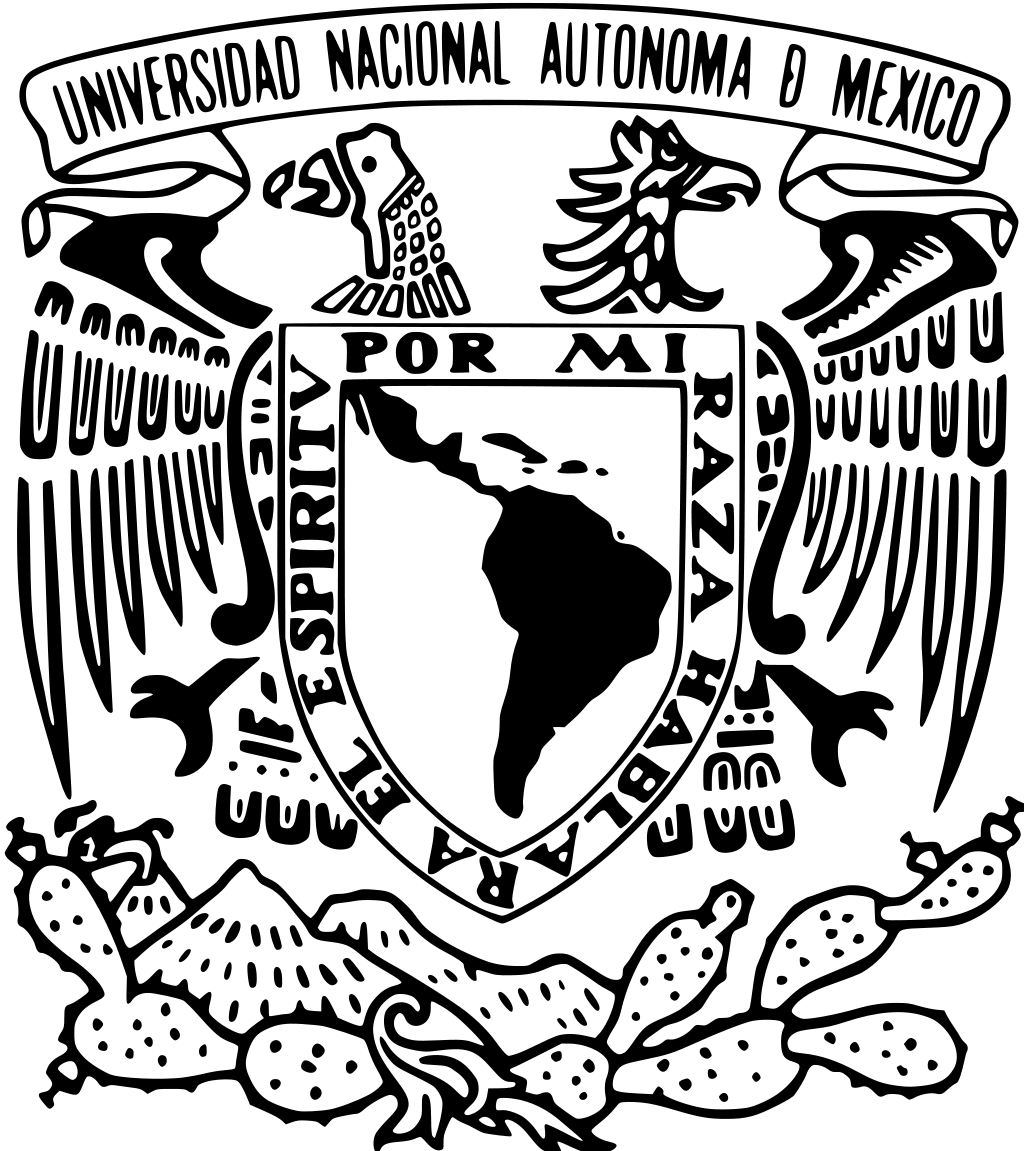
\includegraphics[width=0.4\textwidth]{unam_logo.png}\par\vspace{1cm}
    {\scshape\Large Universidad Nacional Autónoma de México \par}
    \vspace{1cm}
    {\scshape\Large Facultad de Ingeniería \par}
    \vspace{1.5cm}
    {\huge\bfseries Arquitectura de Computadoras \par}
    \vspace{2cm}
    {\Large\itshape David Rivera Morales\par}
    \vfill
    {\large \today\par}
\end{titlepage}

\end{document}


\newpage
\title{Tarea 1}
\author{David Rivera Morales, Christian Eulogio Sánchez}

\maketitle
\section*{Respuestas}


\section*{Pregunta 1}
Expresar -31 y +31 en 8 bits en el sistema de complemento a 1.

\subsection*{Respuesta}
Para el número +31 en 8 bits:

\[
+31 = 00011111_{2}
\]

Para el número -31 en 8 bits usando el sistema de complemento a 1:

\[
-31 = 11100000_{2}
\]

\section*{Pregunta 2}

\subsection*{Respuesta}
Para +13:
\begin{align*}
\text{Valor decimal} & : +13 \\
\text{Binario} & : 1101 \\
\text{Completar 8 bits} & : 00001101 \\
\end{align*}

Para -13:
\begin{align*}
\text{Valor decimal} & : -13 \\
\text{Binario} & : 1101 \\
\text{Completar 8 bits} & : 00001101 \\
\text{Complemento a 1} & : 11110010 \\
\text{Sumar 1} & : 11110010 + 1 = 11110011 \\
\end{align*}

\section*{Pregunta 3}
¿Cuál es el rango de números representables en complemento a dos con 4 bits?

\subsection*{Respuesta}
El rango de números representables en complemento a dos con 4 bits es:
\begin{itemize}
\item Número negativo más pequeño: -8 \quad (\text{equivalente binario}: 1000_2)
\item Número positivo más grande: +7 \quad (\text{equivalente binario}: 0111_2)
\end{itemize}

Por lo tanto, el rango total es de -8 a +7.

\section*{Pregunta 4}
El número \((10110101)_2\) es un número de 8 bits incluyendo el bit de signo en complemento a 2.
Da su equivalente en base decimal.

\subsection*{Respuesta}
El equivalente en base decimal es -75.

\section*{Pregunta 5}
El número \((00110111)_2\) es un número de 8 bits incluyendo el bit de signo en complemento a 2.
Da su equivalente en base decimal.

\subsection*{Respuesta}
El equivalente en base decimal es 55.

\section*{Pregunta 6}
Menciona las cuatro unidades funcionales principales de una computadora y describe su funcionamiento.

\subsection*{Respuesta}
Las cuatro unidades funcionales principales de una computadora son:

\begin{enumerate}
    \item \textbf{Unidad de Procesamiento Central (CPU)}: Es el "cerebro" de la computadora, donde se realizan los cálculos y se maneja la lógica.Incluye la Unidad de Control (CU) que gestiona el flujo de datos y la Unidad de Aritmética y Lógica (ALU) que ejecuta operaciones matemáticas y lógicas.
    
    \item \textbf{Unidad de Memoria}: Almacena temporalmente los datos y las instrucciones que la CPU necesita durante la ejecución de los programas. La memoria principal o RAM es volátil y proporciona un acceso rápido para la CPU.
    
    \item \textbf{Unidad de Entrada}: Compuesta por dispositivos como el teclado, el ratón y el escáner, esta unidad permite al usuario ingresar datos e instrucciones a la computadora.
    
    \item \textbf{Unidad de Salida}: Incluye dispositivos como monitores e impresoras que la computadora usa para comunicar los resultados de sus operaciones al usuario.
\end{enumerate}

\section*{Pregunta 7}
Realiza la siguiente operación \(-3 - 6\) de base decimal en base binario representando los números en 4 bits.
\subsection*{Respuesta}
\begin{align*}
  &\phantom{-}1101_{(2's\ complem.)} \\
  &+1010_{(2's\ complem.)} \\
  \cline{1-2}
  &0111_{2} \text{ (desbordamiento, fuera del rango de 4 bits)}
\end{align*}


\section*{Pregunta 8}
Realiza la siguiente operación \(9 + 3\) de base decimal en base binaria representando los números en 4 bits.
\subsection*{Respuesta}
\begin{align*}
  &\phantom{+}1001_2 \\
  &+0011_2 \\
  \cline{1-2}
  &1100_2
\end{align*}


\section*{Pregunta 9}
Realiza la siguiente suma de 2 bits.
\subsection*{Respuesta}
\begin{align*}
\begin{tabular}{ccc|c|c}
\hline
\multicolumn{1}{|c|}{A} & + & B & Acarreo & Suma \\ \hline
\multicolumn{1}{|c|}{0} & + & 0 & 0       & 0    \\ \hline
\multicolumn{1}{|c|}{0} & + & 1 & 0       & 1    \\ \hline
\multicolumn{1}{|c|}{1} & + & 0 & 0       & 1    \\ \hline
\multicolumn{1}{|c|}{1} & + & 1 & 1       & 0    \\ \hline
\end{tabular}
\end{align*}


\section*{Pregunta 10}

Suma los siguientes dos números $(10011011)_2$ y $(11101100)_2$. Explica qué sucede con el acarreo.

\subsection*{Respuesta}

La suma de dos números binarios se realiza de derecha a izquierda, al igual que en la suma decimal. Cuando la suma de dos bits es 2 (10 en binario), se produce un acarreo.

Consideremos la suma de los números binarios $(10011011)_2$ y $(11101100)_2$:

\begin{align*}
  &\phantom{+}10011011 \\
  &+11101100 \\
  \cline{1-2}
  &110000111
\end{align*}

Vamos a desglosar el proceso:

\begin{itemize}
  \item Empezamos desde la derecha. La suma de los primeros bits es 1 + 0 = 1.
  \item En la segunda posición, la suma es 1 + 0 = 1.
  \item En la tercera posición, la suma es 0 + 1 = 1.
  \item En la cuarta posición, la suma es 1 + 1. Esto es igual a 2, que se representa como 10 en binario. Por lo tanto, escribimos 0 y llevamos 1 al siguiente bit.
  \item En la quinta posición, la suma es 0 (del bit) + 1 (del acarreo) + 0 (del siguiente bit) = 1.
  \item Continuamos este proceso hasta el final.
\end{itemize}

Por lo tanto, el acarreo comienza en la cuarta posición desde la derecha.




\section*{Pregunta 12}

Representa el número 576.65 en base 2 usando el estándar IEEE 754.

\subsection*{Respuesta}

\begin{figure}[H]
    \centering
    \includegraphics[width=\textwidth]{20240229_20h49m03s_grim.png}
    \caption{Simple precisión (32 bits):}
    \label{fig:enter-label1}
\end{figure}

\begin{figure}[H]
    \centering
    \includegraphics[width=\textwidth]{20240229_20h49m13s_grim.png}
    \caption{Doble precisión (64 bits):}
    \label{fig:enter-label2}
\end{figure}

\section*{Pregunta 14}

La Arquitectura Von Neumann fue descrita por el matemático y físico John von Neumann y otros, en el primer borrador de un informe sobre el EDVAC. Pero la computación de 1945 a la actualidad ha dado pasos agigantados, aumentando la complejidad de la arquitectura inicial, la base de su funcionamiento es la misma. ¿Qué cambios aprecias hoy en día en tu computador que no se ven descritos por el diagrama dado en 1945? Argumenta tu respuesta.

\subsection*{Respuesta}

Resumen de los cambios en la arquitectura Von Neumann desde 1945:

\textbf{Memoria:}

\begin{itemize}
  \item Capacidad: Aumento exponencial (de KB a GB/TB).
  \item Velocidad: Acceso más rápido a datos.
  \item Jerarquía: Niveles de memoria (caché, RAM, disco duro) para optimizar rendimiento.
\end{itemize}

\textbf{Procesador:}

\begin{itemize}
  \item Velocidad: Aumento considerable (de MHz a GHz).
  \item Paralelismo: Múltiples núcleos y unidades de procesamiento.
  \item Especialización: Procesadores para tareas específicas (gráficos, aprendizaje automático).
\end{itemize}

\textbf{E/S:}

\begin{itemize}
  \item Dispositivos: Mayor variedad (teclados, ratones, pantallas, impresoras).
  \item Velocidad: Mayor velocidad de transferencia de datos (redes de alta velocidad).
\end{itemize}

\textbf{Software:}

\begin{itemize}
  \item Sistemas operativos: Más complejos, mayor seguridad, estabilidad y facilidad de uso.
  \item Aplicaciones: Crecimiento exponencial (de programas de cálculo a juegos complejos e interfaces multimedia).
\end{itemize}

\textbf{Conclusión:}

La arquitectura Von Neumann ha evolucionado considerablemente desde 1945, adaptándose a las necesidades de la computación moderna. Aunque el diagrama original no describe estos cambios, la base fundamental de la arquitectura se mantiene intacta.

\section*{Pregunta 15}
En la siguiente imagen, se nos muestra la disyuncion y la conjuncion proposicional usando interruptores. Usando ese mismo modelo, como seria un xor usando interruptores?

\begin{figure} [H]
    \centering
    \includegraphics[width=0.75\linewidth]{1641d493-e39b-4626-b583-42ef2d0b38d2.jpeg}
    \caption{xor ejemplo}
    \label{fig:enter-label}
\end{figure}

\end{document}
